%%%
\section{Premises of a LUC OS: The \discovery Proposal\label{sec:archi}}

In this section, we propose to go one step further by discussing preliminary
investigations around the design and the implementation of a first LUC OS
proposal: the \discovery system (DIStributed and COoperative Management of
Virtual EnviRonments autonomouslY). We draw the premises of the \discovery
system by emphasizing some of the challenges as well as some research directions
to solve them. Finally, we give some details regarding the prototype that is
under development and how we are going to evaluate it.  

\subsection{Overview}

The \discovery system relies on a multi-agent peer-to-peer system deployed on
each physical resource composing the LUC infrastructure. Agents are autonomous
entities that collaborate to efficiently use the LUC resources. In our context,
efficiency means that a good trade-off is found between satisfying user's
expectations, ensuring reliability, reactiveness as well as availability of the
services while limiting the energy consumption of the system and providing
scalability. We propose thus to leverage P2P techniques, that
allow self-* properties, such as self-adaptation and self-repairing of overlays. 
%
To reduce the management complexity as well as the design and the
implementation of the different mechanisms that are mandatory, we strongly
support to use micro-kernel concepts. Such an approach should enable to design
and implement services at higher level while leveraging P2P mechanisms
at the lower ones.  Furthermore, to address the different objectives and reduce
the management complexity, we also underline that self-* properties should be
present at every level of the system.  We think that relying on a multi-agent
peer-to-peer system is the best solution to cope with the scale as well as the
network disconnections that may create temporary partitions in a LUC platform.

In \discovery, each agent has two purposes: (i) maintaining knowledge base on the
LUC platform composition (ii) ensuring the correct execution of the VEs. 
Concretely, the knowledge base will consist of overlays that will be used 
for the autonomous management of the
VEs life cycle. This includes the configuration, deployment and monitoring of
VEs as well as the dynamic allocation or relocation of VMs to adapt to changes
in VEs requirements and physical resources availability. To this end, agents
will need to rely on dedicated mechanisms that can be classified as follows: 

\begin{itemize}
\item Mechanisms related to physical resource localization and monitoring, 
\item Mechanisms related to VEs management, 
\item Mechanisms related to the VM images management, 
\item Mechanisms related to reliability,
\item Mechanisms related to security and privacy.
\end{itemize}

\subsection{Resource Localization and Monitoring Mechanisms\label{ssec:p2p}}

Keeping in mind that \discovery should be designed in a fully distributed way,
most of the mechanisms should build on top of overlays in order to abstract changes
that occur at the physical levels. The specific requirements of this platform
will lead to develop a particular kind of overlays, having minimalism in mind.

More concretely, the first step is to design, at the lowest level, a first
overlay layer intended to abstract out the details of the physical routes and
computing utilities, while satisfying the basic topology requirements needed --
locality and availability. This overlay needs to enable the communications
between any two nodes in the platform. While overlay computing has been
extensively studied over the last decade, we emphasize here on minimalism, and
one particular feature with regard to the envisioned platform described before:
retrieving physically close nodes from a given starting node.

\subsubsection*{Giving nodes a position}

The physical network's connections are considered as arbitrary. We choose to
rely on the Vivaldi protocol~\cite{dabek:2001:sigcomm04}. Vivaldi is a
distributed algorithms assigning coordinates in the plane to nodes of a
distributed systems, each node being equipped with a \emph{view} of the network,
\emph{i.e.}, a set of nodes it knows. This view is initially assumed as
arbitrary. Coordinates obtained by a node reflects its \emph{position} in the
network, \emph{i.e.}, close nodes in the network are given close coordinates in
the plane. This is achieved by every node periodically checking the round trip
time between itself and another node (from its view, a different one at each
step) and adapting its distance (by changing its coordinates) with this node in
the plane accordingly. 

\begin{figure}
  \begin{minipage}[c]{.45\linewidth}
	\vspace*{.5cm}
   \hspace*{-0.5cm}
      	\centering 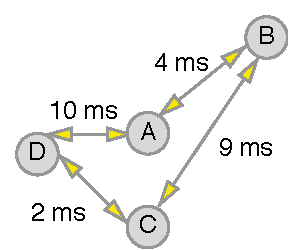
\includegraphics[width=4cm]{./FIGS/vivaldi_before.pdf}

   \hspace*{0.5cm}
	\vspace*{.4cm}
		\caption{Vivaldi plot before updating positions.}
		{\small Each node ping other nodes. Each node maintains a map of distance.}
\label{fig:vivaldi_before}
   \end{minipage}
\hspace*{0.6cm}
   \begin{minipage}[c]{.45\linewidth}
   	\centering 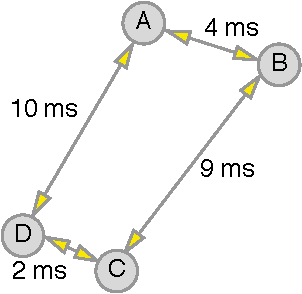
\includegraphics[width=4cm]{./FIGS/vivaldi_after.pdf}
	\vspace*{0.20cm}
		\caption{Vivaldi plot after updating positions.}
		\label{fig:vivaldi_after} 
{\small The computed positions of other nodes are periodically updated.}
  \end{minipage} \hfill
\end{figure}

\newpage

Note that a global accurate positioning of nodes can be
obtained if nodes have a few long-distance nodes in their
view~\cite{dabek:2001:sigcomm04}. These long distance links can be easily
maintained through a simple gossip protocol.

\subsubsection*{Searching for close nodes}

Once this map is achieved (each node its coordinates), we are able to decide
whether two nodes are close by calculating their distance. However, the view of
each node does not \emph{a priori} contain its closest nodes. We need additional
mechanisms to locate a set of nodes that are close to a given initial node --
Vivaldi gives a \emph{location} to a node, but not a neighborhood. To achieve
this, we use a modified distributed version of the classic Dijkstra's algorithms
used to find the shortest path between two nodes in a graph. The goal is to
build a \emph{spiral}\footnote{The term \emph{spiral} is here a misuse of
language, as there is no guarantee that the graph actually drawn in the plane
does not contain crossing edges. The only guarantee is that when following the
path constructed, the nodes are always further from the initial node.}
interconnecting the nodes in the plane that are closest to a given initial
node. Let us consider our starting point is node $s$. The first step is to find
a node to build a two-node spiral with $s$. Such a node is sought in the current
view of $s$ by selecting the node, say $a$, having the smallest distance with
$s$. By contacting $a$, $s$ then sends its view to $a$, $s$ stores $a$ as its
successor in the spiral, and $a$ adds $s$ as its predecessor in the spiral. Then
$s$ forwards its view to $a$. $a$ then creates a new view by keeping the $n$
node which are closest to $a$ in both $s$ and $a$'s views. This last view is
then referred to as the \emph{spiral view} and is intended to contain a set of
nodes in which to find the next step of the spiral. Then $a$ restarts the same
process: Among the spiral view, it chooses the node with the smallest distance
to $s$, say $b$, and adds it in the spiral -- $a$ becomes the predecessor of $b$
and $b$ becomes the successor of $a$. Then, the spiral view is sent to $b$ which
updates it with the nodes it has in its own view. The process is repeated until
we consider we have gathered enough nodes with regard to the requesting
application.

One risk to be mitigated is not to blocked by a spiral view containing only
nodes that are already in the spiral. However, this problem can be easily
addressed by forcing the presence of a few long distance nodes whenever it is
updated.

\subsubsection*{Learning}

Applying the protocol described above, the quality of the spirale is
questionable in the sense that the nodes that are actually close to the starting
point node $s$ may not be included. The only property ensured is that one step
forward the path built always takes us further from the starting point node.

To improve the \emph{quality} of the spiral, \emph{i.e.}, reduce the average
distance between the nodes it comprises and the initial node, we add a learning
mechanism coming with no extra communication cost, as it does not require any
extra message. When a node is contacted for becoming the next node in one
spiral, and receives the associated spiral view, it can also keep the nodes that
are closest to itself, thus potentially increasing the quality of a future
spiral construction.

\subsubsection*{Routing}

In the context of a LUC infrastructure, one crucial feature is to be able to
locate an existing VM. Having the same stratery consisting in improving the
performance of the overlay based on the application's activity, we envision a
routing mechanism which will be improved by past routing requests. Thanks to the
spiral mechanism described above, a node is able to contact its neighbouring
nodes to start the path of a message.

This initial routing mechanism can be very expensive, as the number of hops can
be linear in the size of the network. From previous communications, one is able
to memorize long links to different locations of the network. Consequently, 

From each routing request, the source of the request and each node on the path
to the destination is able to learn long links, which will significantly reduce
the number of hops of future requests. We currently study the amount of requests
needed to approach a logarithmic routing complexity.

More generally, we work on the estimation of the application's activity required
to (i) guarantee the constant efficiency of the overlay, (ii) converge, started
from a random configuration, to a fully-efficient overlay network.

%\ftodo[CT]{TODO}

% Each node doing so in parallel, a number of clusters are created inside which we
% can ensure a certain level of locality -- all nodes inside this group can
% communicate with each other very efficiently. Given the number of nodes in these
% groups, the inner topology of a group can either rely on very simple graphs,
% such as rings, or more connected graphs, to accelerate the dissemination and
% retrieval of information in the group. Note that, still based on simple
% gossiping techniques, such graphs can be easily maintained as the network's
% conditions change. For instance, if a link becomes overloaded, the other nodes
% will react to this change by removing nodes with which they communicate through
% this link from their local group. Such groups are exemplified on
% Figure~\ref{fig:renater_overlay} (for the west part of the platform).

% \begin{figure}[htbp]
% 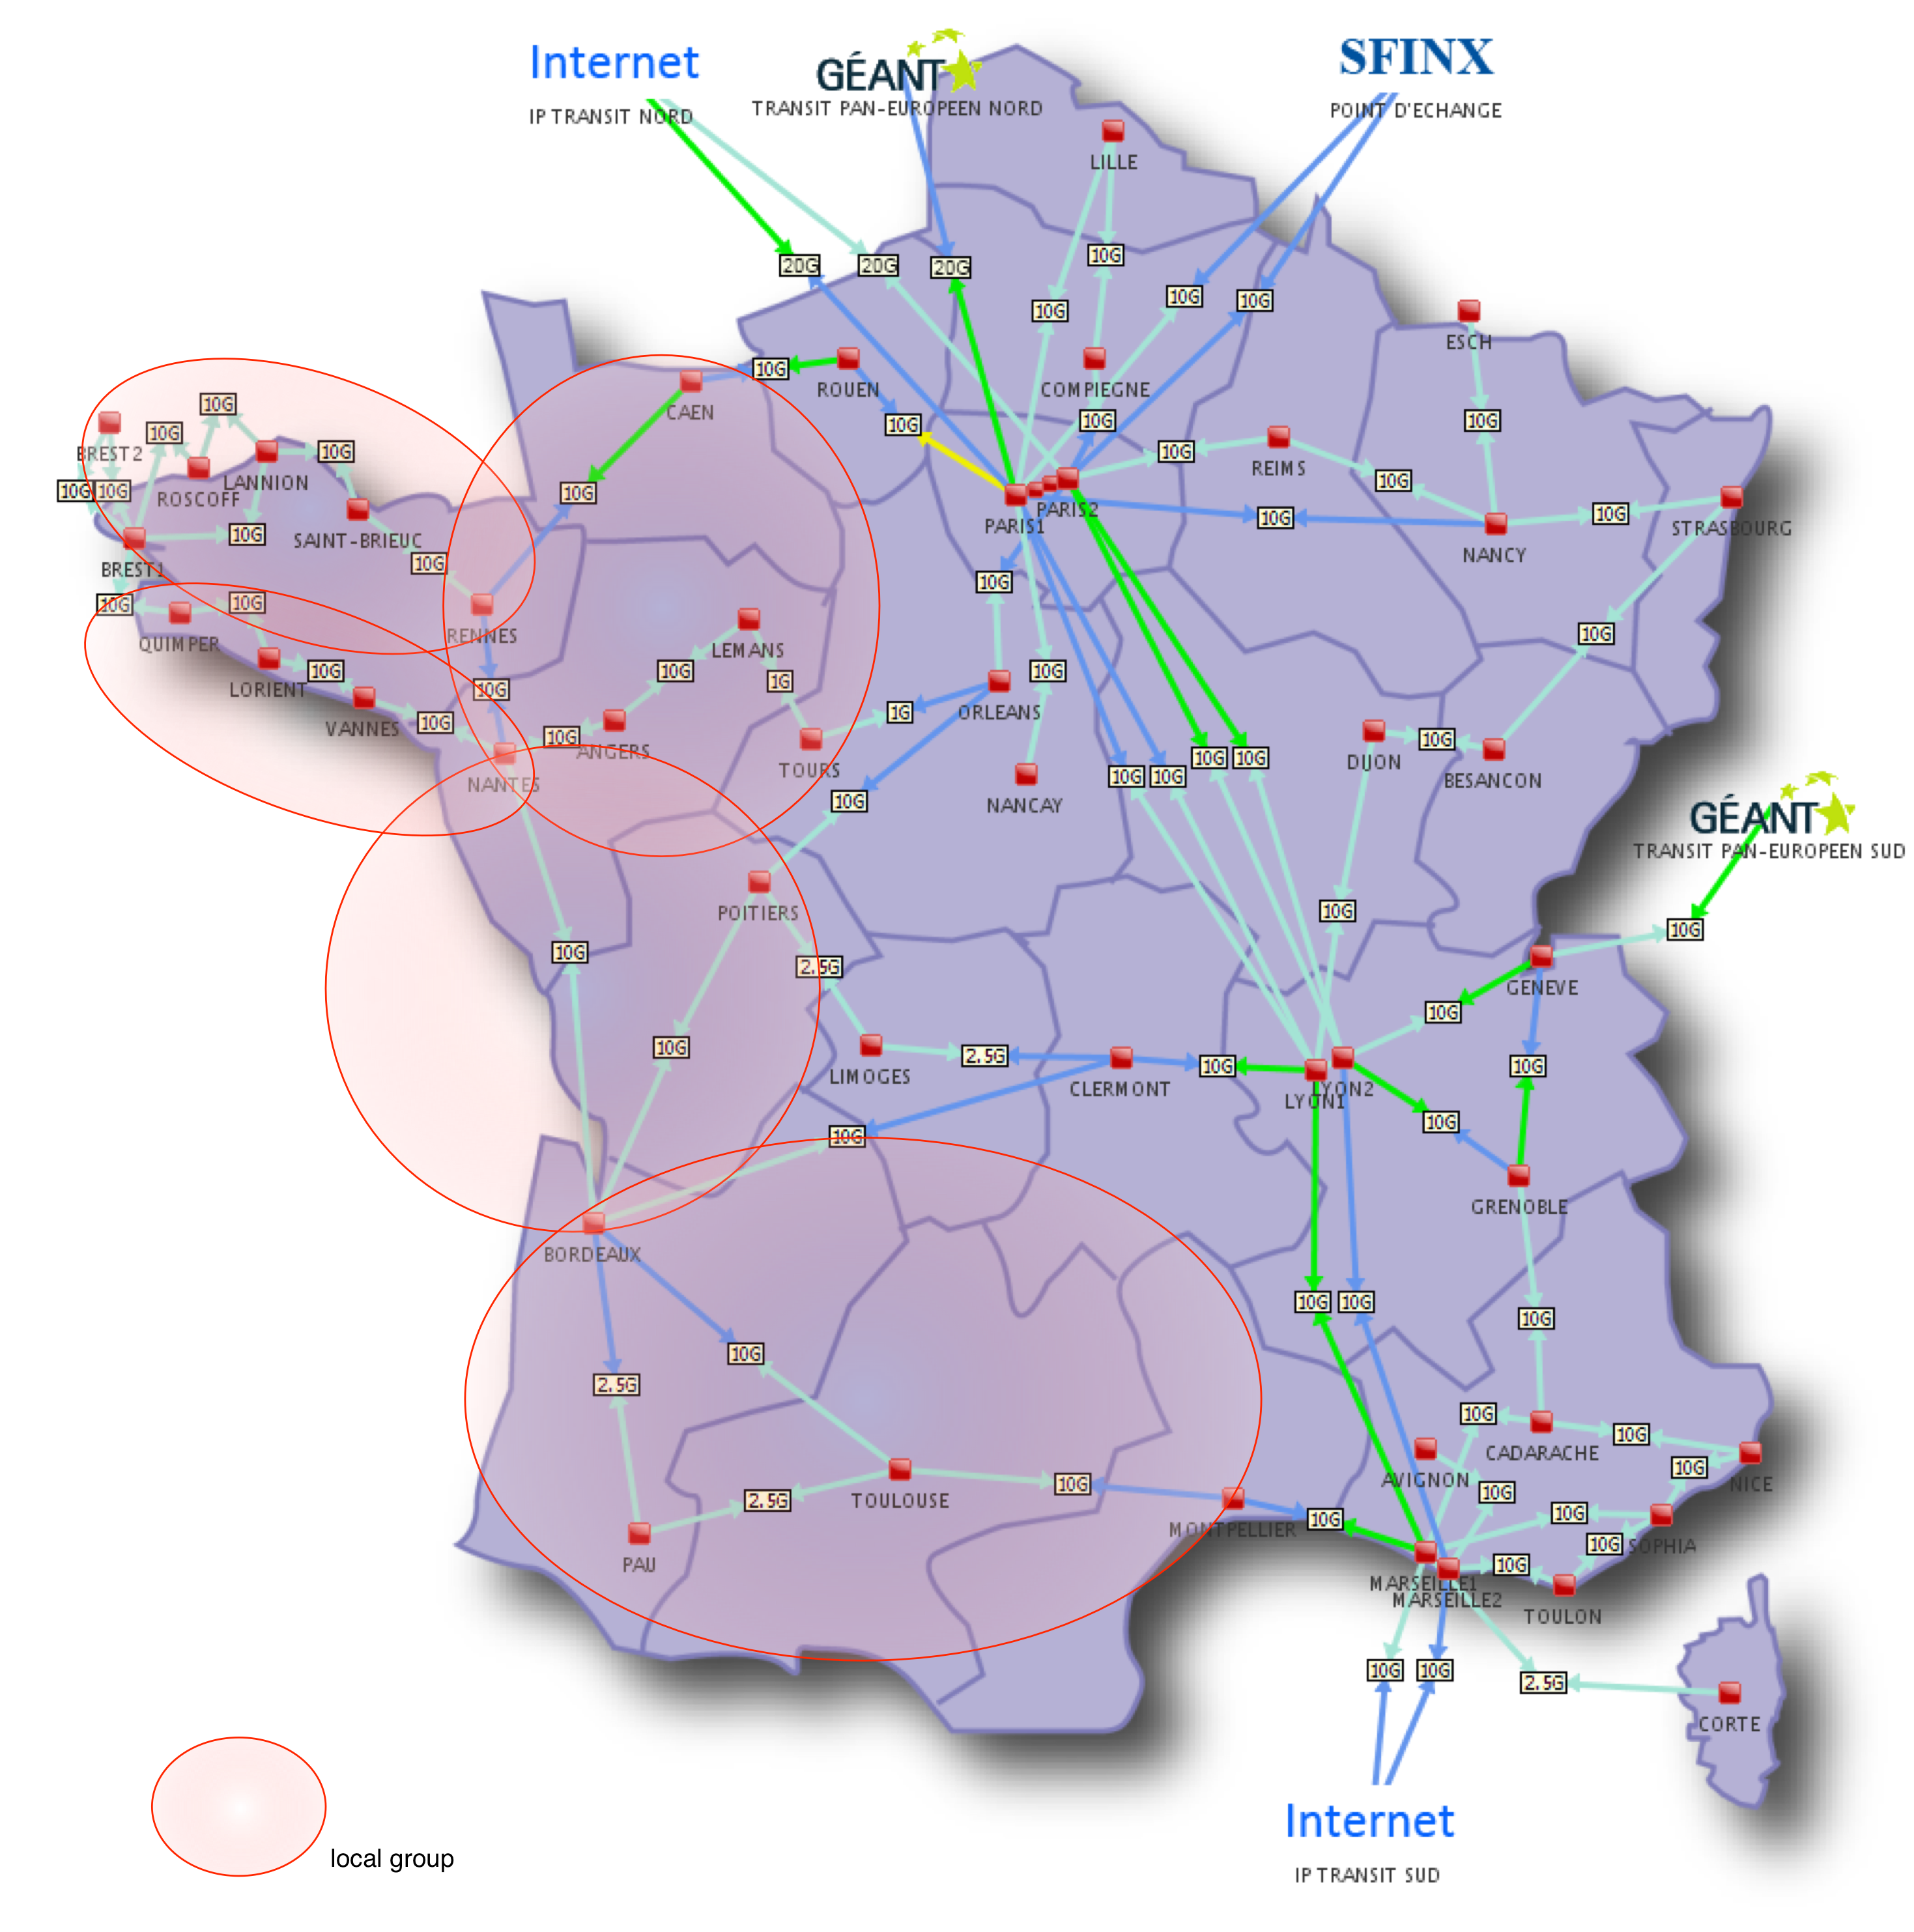
\includegraphics[width=12cm]{./FIGS/renater_overlay.png}
% \caption{Overlay local groups on top of the RENATER platform.\label{fig:renater_overlay}}
% \end{figure}

% As we can see on Figure~\ref{fig:renater_overlay}, it follows from the way the
% overlay is built that some nodes may be a member of several groups. The Nantes
% site for instance is part of three of these groups, given its
% physical position. More generally, the overlay will take the shape of a set of
% groups with some \emph{bridges} between the groups. Note that several
% \emph{bridges} can interconnect two local groups. Thus, any request first goes
% through local nodes allowing for its local processing, and avoiding the need for
% global coordination mechanisms.

% To be able to localize a particular VM, the system has to be able to route a
% request from any node to any other node. This functionality is the classic
% problem of P2P overlays, which is traditionally solved in structured overlay networks by
% maintaining a routing table on each node, and by a flooding mechanism or with
% random walks in unstructured overlays. These techniques are usually designed for
% very large scale networks with different guarantees and costs. Here, given the
% particular ``intermediate'' scale of the platform, and its specific
% requirements, we believe that these existing techniques are too
% \emph{powerful}. As we want to design a minimalistic overlay, there is room to
% try to design a new routing technique specifically fitting our
% requirements. The aim is then to maintain, in all groups, information about the
% distance between this group and \emph{close} groups in terms of number of bridge nodes
% to go through. Hence, the system will be able to route quickly between \emph{close}
% groups. The routing of requests between \emph{far} groups will be based on a random
% decision when no information are available, but \emph{oriented} by the aim of
% going away from the request's source.

% This overlay will provide the basic building block of the platform, on which will
% rely higher level overlays and functionalities, which are described in the
% following sections.

% \subsubsection*{Upper-Layer overlays}

% \ftodo[CT]{To be completed...}


% \ftodo[AL]{To be completed by Cedric and Marin}
% \ftodo[AL]{C/P from the proposal : 
% self-organizing overlay construction mechanisms based on gossip and epidemic
% techniques that will link the \discovery resources in navigable graphs onto
% which requests for VE can be routed and allocated. It will investigate
% mechanisms to quickly adapt these graphs to changing conditions and
% infrastructure, and mechanisms to monitor the adequacy of previous requests
% solutions to these changing conditions as these occur.}

\subsection{VEs Management Mechanisms}
\label{ssec:vem}
In the \discovery system, we define a VE as a set of VMs that may have specific
requirements in terms of hardware, software and also in terms of placement:~
some VMs must be on the same node/site in order to cope with performance objectives while
others should not be collocated in oder to ensure
high-availability criteria~\cite{hermenier:2013}.
As operations on a VE may occur in any place from any location, each agent should provide the capability
to configure and start a VE, to suspend/resume/stop it, to relocate some of its VM if need be or simply to retrieve the location of a particular VE. 
Most of these mechanisms are integrated on current UC platforms. However as mentioned, they
should be revisited to correctly run on the infrastructure we target
(\textit{i.e.} in terms of scalability, resiliency and reliability).
To this aim, the \discovery system relies on the aforementioned P2P mechanisms. 
As a first example, placing the VMs of a VE requires to be able to find available nodes that
fulfills the VM needs (in terms of resource needs as well as placement
constraints). Such a placement can start locally, close to the client
application requesting it, \textit{i.e.}, in its local group. If no such node is
found, simple navigation ensures that the request will encounter a bridge
eventually, leading to the exploration of further nodes. This navigation goes
on until one sufficiently available node is found.
A similar process is performed by the mechanism in charge of  dynamically
controlling and adapting the placement of VEs during their lifetime.  For instance, in
order to ensure particular needs of a VM, it can be necessary to relocate other
ones. According to the predefined constraints of VEs, some VMs might be
relocated on far nodes while other would prefer to be suspended.  Such a
mechanism has been deeply studied and validated in the DVMS
mechanism~\cite{dvms:wiki,quesnel:2012}. DVMS (Distributed Virtual
Machines Scheduler) enables to dynamically schedule a significant number of VMs
throughout a large-scale distributed infrastructure while guaranteeing VM
resource expectations.  

A second example regards the configuration of the network elements of a VE. 
Although it might look simple, assigning the right IPs to
each VM as well as maintaining the intra-connectivity of a VE becomes a bit more complex than in
the case of a single network domain, \textit{i.e.} a mono-site deployment.
%
Keeping in mind that a LUC infrastructure is
by definition spread WANwide, a VE can be hosted between distinct network
domains during its lifetime. No solution has been chosen yet. 
Our first investigations led us to leverage techniques
such as the IP over P2P project \cite{ganguly:2006}. However, the definition of
software network becomes more and more important. Investigating proposals such as
the Open vSwitch project \cite{pfaff:2009} looks a promising direction to solve such issue.
%

\subsection{VM Images Management}

In a LUC infrastructure, VM images could be deployed in any place from any
other location, but being in a large-scale, heterogeneous and widely spread
environment makes the management of VM images more difficult than more
conventional  centralized repositories.  
At coarse grain, the management of the VM images should be (i) consistent
with regards to the location of each VM throughout the \discovery infrastructure and
(ii) reachable in case of failures.
%
The envisioned mechanisms dedicated to the management of the VM images have been
classified into two sub-classes.
%
First, it will be mandatory to deliver appropriate mechanisms to efficiently
upload and replicate VM images among a high number of nodes in order to ensure
efficiency as well as reliability.  Second, the \discovery system should 
include specific mechanisms devoted to the scheduling of the VM image
transfers. Advanced policies are important to improve the efficiency of each
transfer that may occur either at the boot time or during VM relocations. 

Regarding storage and replication mechanisms,  an analysis of an IBM Cloud concludes
that a fully distributed model using P2P technology is not the best choice to manage VM images as the
number of instances of the same VM image is rather small~\cite{peng:2012}. However, central or
hierarchical solutions are not suited for the infrastructure we target.
Consequently, an augmented P2P solution working with replicas and
deduplication will have to be investigated in order to provide more
reliability, speed, and scalability to the system. For example, analyzing
different VM images shows that at least 30\% of the image is shared between
different VMs. This 30\% can become a 30\% space reduction, a
30\% increased reliability or a 30\% of speed increase. Depending on the
situation, we should decide to go from one scenario to another. 
%Finally, the number of replicas and deduplicated data should be dynamically balanced.

Regarding the scheduling mechanisms, it has been shown that a storage system with VMs being used by I/O intensive tasks 
can increase boot time from 10 to 240 seconds \cite{tan:2008}. Some actions like providing the
image chunks needed to boot first~\cite{tang:2011}, defining a new
image format, and pausing the rest of the I/O operations, can provide a
performance boost and limit the overhead that is still observed in commercial
Clouds~\cite{mao:2012}. 
%These actions should also take into account
%power-like metrics in order to reduce the energy consumption of data transfers.
%According to (Preist et Shabajee Nov 2010) the cost to transmit 1 MB can be of
%4Wh. Considering the size of VM images, any improvement aiming at reducing
%data movement will make a big difference.

More generally, the amount of data related to VM images is significant.
Actions involving data  should be aware of their implications on metrics like
(but not limited to): energy efficiency, bandwidth, reliability, proximity, and
hardware usage. The scheduler could also anticipate actions like moving images when
the load is low or the energy is cheaper.

%% \subsection{Reliability Mechanisms}
%% %These mechanisms should ensure  reliability and high availability of the
%% %\discovery system despite the scale and dynamicity of the underlying physical
%% %infrastructure.   
%% By nature, a LUC is a highly distributed platform where 
%% node and network failures will be much more frequent than in
%% actual UC platforms.  Furthermore, since resources could be located anywhere,
%% the expected mean time to repair failed equipments might be much larger than in
%% other platforms. For all these reasons, a set of dedicated mechanisms should be designed in order
%% to provide a fully transparent failure management with minimum downtime. 
%% %
%% To this aim, the \discovery system should include, first,  mechanisms in charge of its own reliability. 
%% Such mechanisms are required to avoid losing or corrupting important information
%% regarding the state of the system.  Of course, handling all kinds of failures
%% and implementing a fully resilient operating system is a complex task. Hence,
%% we propose to consider in a first time a crash-stop failure model. In other words, the
%% \discovery system should be able to autonomously restart any service by
%% relocating it on an healthy agent each time it is mandatory.  This implies to
%% define a common design pattern, \textit{i.e.} a set of recommendations, that each
%% service should follow to ensure such characteristics. Besides, in order to
%% ensure that such a pattern may be applied to stateful services, the system can
%% require a Cassandra like system \cite{lakshman:2010} that provides reliable and highly available
%% storage for critical system states. Retrieving the information related to one
%% service need to rely on the kind of mechanisms described in Section~\ref{ssec:p2p}.

%% %
%% In addition to be robust enough, the \discovery system should ensure the
%% reliable execution of virtual environments. The first mechanisms consists in
%% using snapshotting capabilities delivering by virtualization technologies.
%% Concretely, each internal states of a VM should be periodically saved on a
%% persistent storage.  When a crash occurs on a VM, its associated VE can be
%% restarted from the latest consistent states, \textit{i.e.} all VMs of the VE will be
%% resume for their latest snapshot.  As for the other mechanisms, performing VM
%% snapshotting in a large-scale, heterogeneous and widely spread environment is a
%% challenging task. However, we believe that aforementioned mechanisms in charge
%% of the VM images as well as recent proposals \cite{nicolae:2011} might enable
%% to provide such a feature. 
%% Although VM snapshotting provides a first level of reliability, it is not
%% sufficient to ensure high availability of the VE. More advanced mechanisms must
%% be proposed.  Our idea is to include mechanisms based on primary-backup
%% replication techniques. 
%% The basic principle is to have one active replica of the VM (the primary)
%% sending state updates to the other replicas (the backups) periodically. If the
%% primary fails, one of the backup can resume the execution transparently for the
%% outside world. Furthermore since the entire VM is replicated, applications can
%% be run unmodified.  Solutions to replicate VMs inside a cluster have been
%% proposed. However efficiently replicating VMs over a WAN is a huge challenge.
%% Limiting the size of the backup updates\cite{rajagopalan:2012}, and
%% reducing the impact of the required synchronizations on the execution of the
%% primary \cite{gerofi:2012}  are research directions to be further
%% studied. A better understanding of the parts of a VM that really need to be
%% updated is required. It might require to trade transparency for performance by
%% allowing latency-sensitive applications to define which part of their state has
%% to be updated.

%% \ftodo[AL]{Integrate the P2P aspect into the reliability section}
%% \subsubsection*{Monitoring Example}

%% Another key use of this low-level overlay is proactive replication of VMs,
%% keeping in mind that two identical VMs should be placed in relatively distant
%% nodes, for fault-tolerance reasons (close nodes have a high probability to fail
%% together). Following the defined overlay structure, this can be done through a
%% navigating scheme where at least one bridge is encountered. Monitoring this
%% replica can be done easily by having a \emph{watcher} in the same local group as
%% the replica.

\subsection{Reliability Mechanisms}
%These mechanisms should ensure  reliability and high availability of the
%\discovery system despite the scale and dynamicity of the underlying physical
%infrastructure.   
In a LUC, failures will be much more frequent than in actual UC
platforms. Furthermore, since resources could be highly distributed,
the expected mean time to repair failed equipments might be much
larger than in other UC platforms. For all these reasons, a set of
dedicated mechanisms should be designed in order to provide fully
transparent failure management with minimum downtime. 

%% It includes
%% mechanisms to ensure the high availability of the \discovery system
%% itself and mechanisms to allow executing VEs reliably.

Ensuring the high availability of the \discovery system requires being able to
autonomously restart any service by relocating it on a healthy agent each time
it is mandatory. To avoid losing or corrupting important information regarding
the state of the system, a Cassandra-like system~\cite{lakshman:2010} is
required to provide a reliable and highly available back-end for stateful
services.

Regarding VEs reliability, a first level of fault tolerance can be
provided by leveraging VMs snapshotting capabilities. Periodical
snapshots will allow restarting the VE from its last snapshot in the
event of a failure. Performing VM snapshotting in a large-scale,
heterogeneous, and widely spread environment is a challenging
task. However, we believe that adapting recently proposed
ideas~\cite{nicolae:2011} in this field would allow us to provide such
a feature.

Snapshotting is not enough for services that should be made highly
available, but a promising solution is to use VM
replication~\cite{Petrovic2012}. To implement VM replication in a WAN,
solutions to optimize synchronizations between
replicas~\cite{gerofi:2012,rajagopalan:2012} should be
investigated. Also, we think that a LUC has the major advantage over
other UC platforms, that it is tightly coupled with the network
infrastructure. As such, we can expect \emph{low} latencies between
nodes and so, to be able to provide strong consistency between
replicas while achieving acceptable response time for the replicated
services. 
%Note that the overlays presented in Section~\ref{ssec:p2p}
%for replicas localization and monitoring. Locating replicas based on a
%navigating scheme where at least one bridge is encountered, would be
%enough to ensure that they have a low probability to fail
%simultaneously.


Reliability techniques will of course make uses of the overlays
for resource localization and monitoring. 
Replicated VMs should be hosted on nodes that have a low
probability to fail simultaneously. Following the previously defined
overlay structure, this can be done through a navigating scheme where
at least one bridge is encountered. Monitoring a replica can then be
done by having a \emph{watcher} in the same local group as the
replica.

%% Another key use of this low-level overlay is proactive replication of VMs,
%% keeping in mind that two identical VMs should be placed in relatively distant
%% nodes, for fault-tolerance reasons (close nodes have a high probability to fail
%% together). Following the defined overlay structure, this can be done through a
%% navigating scheme where at least one bridge is encountered. Monitoring this
%% replica can be done easily by having a \emph{watcher} in the same local group as
%% the replica.




%
%% To this aim, the \discovery system should include, first,  mechanisms in charge of its own reliability. 
%% Such mechanisms are required to avoid losing or corrupting important information
%% regarding the state of the system.  Of course, handling all kinds of failures
%% and implementing a fully resilient operating system is a complex task. Hence,
%% we propose to consider in a first time a crash-stop failure model. In other words, the
%% \discovery system should be able to autonomously restart any service by
%% relocating it on an healthy agent each time it is mandatory.  This implies to
%% define a common design pattern, \textit{i.e.} a set of recommendations, that each
%% service should follow to ensure such characteristics. Besides, in order to
%% ensure that such a pattern may be applied to stateful services, the system can
%% require a Cassandra like system \cite{lakshman:2010} that provides reliable and highly available
%% storage for critical system states. Retrieving the information related to one
%% service need to rely on the kind of mechanisms described in Section~\ref{ssec:p2p}.

%% %
%% In addition to be robust enough, the \discovery system should ensure the
%% reliable execution of virtual environments. The first mechanisms consists in
%% using snapshotting capabilities delivering by virtualization technologies.
%% Concretely, each internal states of a VM should be periodically saved on a
%% persistent storage.  When a crash occurs on a VM, its associated VE can be
%% restarted from the latest consistent states, \textit{i.e.} all VMs of the VE will be
%% resume for their latest snapshot.  As for the other mechanisms, performing VM
%% snapshotting in a large-scale, heterogeneous and widely spread environment is a
%% challenging task. However, we believe that aforementioned mechanisms in charge
%% of the VM images as well as recent proposals \cite{nicolae:2011} might enable
%% to provide such a feature. 
%% Although VM snapshotting provides a first level of reliability, it is not
%% sufficient to ensure high availability of the VE. More advanced mechanisms must
%% be proposed.  Our idea is to include mechanisms based on primary-backup
%% replication techniques. 
%% The basic principle is to have one active replica of the VM (the primary)
%% sending state updates to the other replicas (the backups) periodically. If the
%% primary fails, one of the backup can resume the execution transparently for the
%% outside world. Furthermore since the entire VM is replicated, applications can
%% be run unmodified.  Solutions to replicate VMs inside a cluster have been
%% proposed. However efficiently replicating VMs over a WAN is a huge challenge.
%% Limiting the size of the backup updates\cite{rajagopalan:2012}, and
%% reducing the impact of the required synchronizations on the execution of the
%% primary \cite{gerofi:2012}  are research directions to be further
%% studied. A better understanding of the parts of a VM that really need to be
%% updated is required. It might require to trade transparency for performance by
%% allowing latency-sensitive applications to define which part of their state has
%% to be updated.

%% \ftodo[AL]{Integrate the P2P aspect into the reliability section}
%% \subsubsection*{Monitoring Example}

%% Another key use of this low-level overlay is proactive replication of VMs,
%% keeping in mind that two identical VMs should be placed in relatively distant
%% nodes, for fault-tolerance reasons (close nodes have a high probability to fail
%% together). Following the defined overlay structure, this can be done through a
%% navigating scheme where at least one bridge is encountered. Monitoring this
%% replica can be done easily by having a \emph{watcher} in the same local group as
%% the replica.


\subsection{Security and Privacy Mechanisms}
%
%LUC OS should include a mechanism for the security of the lower layers and particularly multiple P2P overlays.
%% Previous research~\cite{sybilattacks} has shown that without trusted identities, it 
%% is not possible to protect a P2P overlay against sybil attacks. 
%Recent advances~\cite{Castro:2002:SRS:844128.844156} in DHT 
%security might enable to provide a secured overlay. 
%But they are not sufficient to ensure the good behavior of resources and users.
%LUC OS should include an authentication and certification mechanism that 
%evaluates the behavior of resources and VEs.
%% Finally, as the resources could be hosted in more or less secured locations and provided by different 
%% resource providers, this certification should also be used to rank the security of each resources.
%% \ftodo[AL->JRC]{Could you please put only the most relevant one}
%
%Moreover, LUC OS shoud integrate security decision and enforcement points (SDEPs).
%%  mechanisms at all locations and layers.
%To guarantee a security, 
%Sandhu~\cite{sandhu_towards_2010} propose a roadmap towards such security mechanisms for
%Cloud where the Cloud infrastructure provides security hooks and
%mechanisms. 
%% To realize this goal, they point out the need for
%% \emph{developing models, methodologies and architectures for
%%   decentralized dynamic management of security and assurance
%%   policies}. 
%Similarly than other mechanisms, 
%As LUC infrastructure is even more distributed, heterogeneous and 
%dynamic than Cloud, its SDEPs should be distributed and 
%decentralized and able to evolve according to security requirements 
%without central security decision points. Futhermore, 
%LUC OS should provide a protocol to ease the collaboration between the SDEPs.
%Indeed, when new resources join
%a LUC infrastructure, SDEPs from different locations 
%must collaborate to extend the LUC infrastructure while keeping it secured. This collaboration between 
%SDEPs will also append when a VE is spread over different 
%resources and/or migrate from one to another.
%
%LUC OS should allow users to express their security requirements on their VEs.
%The expression of these requirements itself is a complex task.
%% LUC OS must propose to the user a way to model their VEs and 
%% the security requirements on them. 
%To ease the expression of these 
%requirements, LUC OS must propose a domain specific security language 
%that defines high-level security requirements such as \cite{rouzaud_book13b,Bacon:2010:EEA:2023718.2023739} do 
%for Clouds. These security requirements will be enforced 
%by SDEPs during the whole life time of the VE.
%
%%%%
% 1./ Securiser les overlays
% 3.a./ Definir  un DSL pour les VEs
% 3.b/ Offrir des moyens d'integrer des SDEPs (i.e. moulinette qui maintient/execute les DSLs)
% 2./ Securiser l'acces aux operations de manipulation de l'infra (admin et user)

% 1
To be successful, \discovery needs to provide mechanisms and methods to construct trust relationships between resource providers.
Trust relationships are known to be complex to build~\cite{Miller:2010:TWT:1907636.1907726}. Providing strong authentication, assurance and certification mechanisms for 
providers and users is required but it is definitely not enough. Trust covers socio-economic aspects that must be covered but are out of the scope of this chapter.
The challenge is to provide a trusted \discovery base.

% 2 
As overlays are fundamentals for all \discovery mechanisms, the first challenge is to ensure
that they are not compromise. Recent advances~\cite{Castro:2002:SRS:844128.844156} might enable to tackle such concerns.

%3.A ? 
The second challenge will consist in providing end-users with a way to define their own  security policies and to ensure that such policies are enforced. 
The expression of these requirements itself is a complex task.
The challenge is to improve the current trade-off between security and usability.
To ease the expression of these policies, we are currently defining a  domain specific security language
that defines high-level security requirements \cite{rouzaud_book13b,alefray:hpdc:2013}. 
These security policies will be enforced in a decentralize manner
by distributed security decision and enforcement points (SDEPs) during the whole lifetime of the VE.
Implementing such SDEP mechanisms in a distributed fashion will require to
conduct specific research as they are currently only prospective proposals for
classic UC infrastructures~\cite{Bacon:2010:EEA:2023718.2023739,sandhu_towards_2010}. 
The challenge will consist in investigating whether such proposals can be adapted to the LUC
infrastructure by leveraging appropriate overlays.
%%  

% Finally, as traditional distributed systems, \discovery should ensure the good behavior of resources and users.
% To this aim, authentication and certification mechanisms should be provided. 

\subsection{Toward a First Proof-of-Concept}

The first prototype is under heavy implementation. It aims at delivering a
simple mock-up for integration/collaboration purposes.  Following the
coarse-grained architecture described in the previous sections, we have
started to identify all the components participating in the system, their
relationships, as well as the resulting interfaces. 
Conducting such a work now is mandatory to move towards a more complete as well
as more complex system. 

To ensure a scalable and reliable design, we  chose to rely on the use
of high-level programming abstractions, more precisely, we are using distributed
complex event programming \cite{janiesch:2011} in association with actors
model \cite{agha:1986}. This enables to easily switch between a push and a pull
oriented model according to our needs. 
%To make the integration of the mechanisms easier, we propose to follow a Service
%Oriented Architecture \cite{valipour:iccsit09}.

Our preliminary studies showed that a common building block is mandatory to
handle resilience concerns in all components. Concretely, it corresponds to a
mechanism in charge of throwing notifications that are triggered by the low
level network overlay each time a node joins or leaves it.  Such a mechanism
makes the design and the development of higher building blocks easier as they do
not have to provide specific portions of code to monitor infrastructure
changes. 

This building block has been designed around the \emph{Peer Actor} concept (see~Figure~\ref{fig:supervisor} and
~\ref{fig:peeractor}).
 The \emph{Peer Actor} serves as an interface between higher services
and the communication layer. It provides methods that enable to define the behaviors of a
service when a resource joins or leaves a particular P2P overlay as well as
when neighbors change.
Considering that several overlays may co-exist through the \discovery system, 
the association between a \emph{Peer Actor} and its \emph{Overlay Actor} is
done at runtime and can be changed on the fly if need be. However, it is noteworthy that 
each \emph{Peer Actor} takes part to one and only one overlay at the same time.  
%
In addition to the \emph{Overlay Actor}, a \emph{Peer Actor}  is composed of a
\emph{Notification Actor}  that processes events and notifies registered actors.
%
As illustrated in Figure~\ref{fig:peeractor}, a service can use more than one \emph{Peer Actor} (and reciprocally). 
Mutualizing a \emph{Peer Actor} enables for instance to reduce the network overhead implied by the overlays' maintenance. 
In the example, the first service relies on a \emph{Peer Actor} implementing a Chord
overlay while the second service uses an additional \emph{Peer Actor} implementing a CAN structure.
 
\begin{figure}
  \begin{minipage}[c]{.35\linewidth}
	\vspace*{2.5cm}
   \hspace*{-0.5cm}
      	\centering 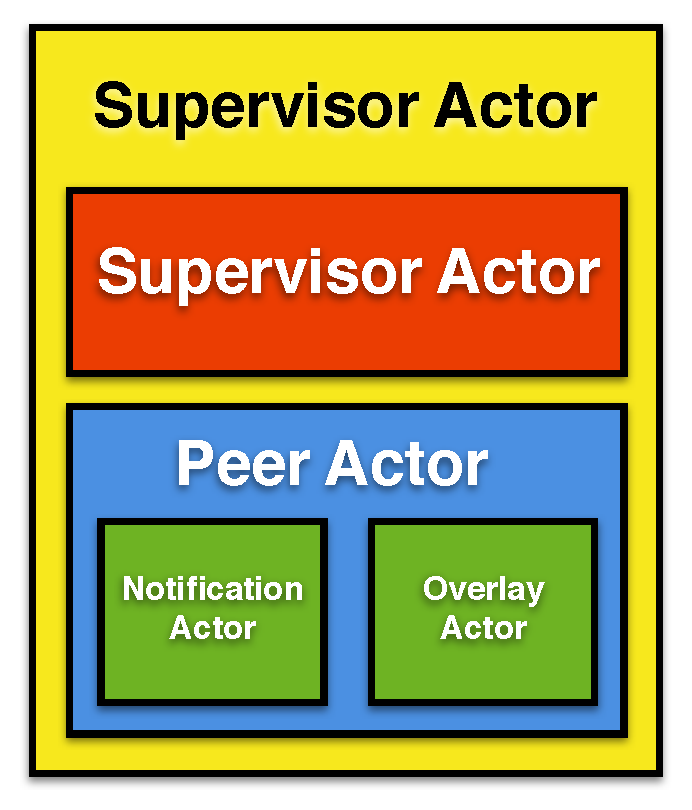
\includegraphics[width=4cm]{./FIGS/PeerActor.pdf}

   \hspace*{0.5cm}
	\vspace*{.8cm}
		\caption{The Peer Actor Model}
		{\small The Supervisor actor monitors all the actors it encapsulates while the Peer actor acts as an interface between the services and the overlay.}
\label{fig:supervisor}
   \end{minipage}
\hspace*{0.6cm}
   \begin{minipage}[c]{.55\linewidth}
   	\centering 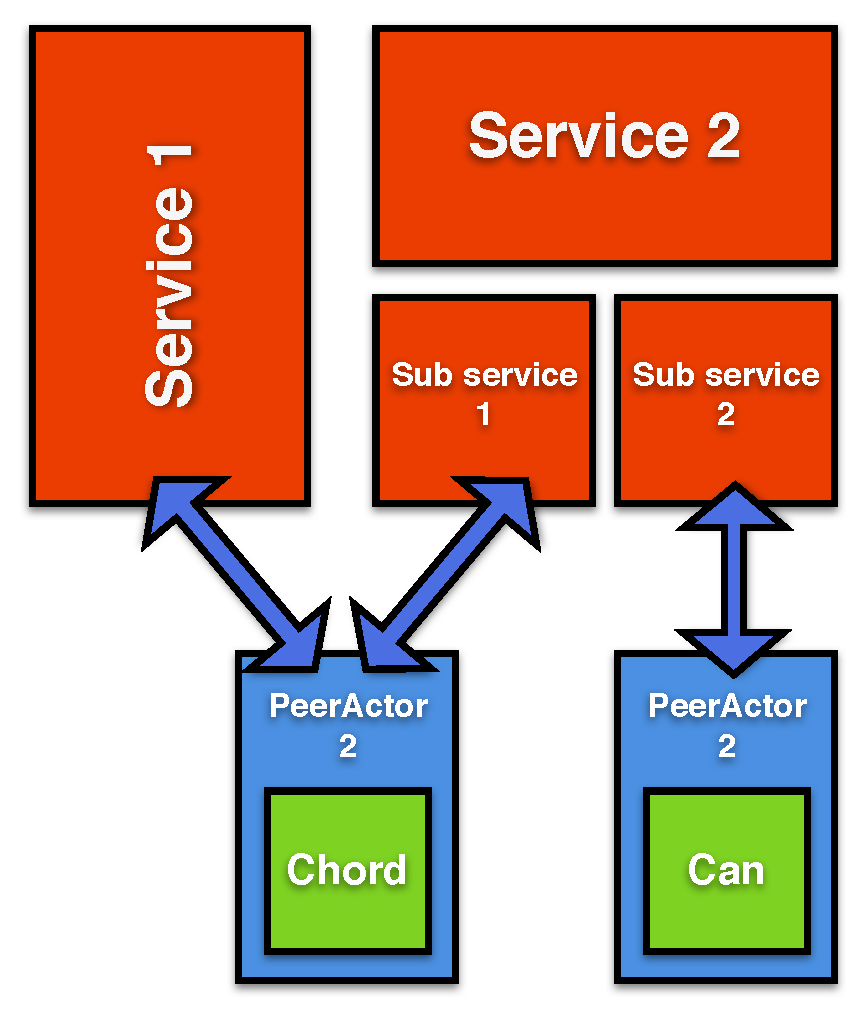
\includegraphics[width=6.5cm]{./FIGS/PeerActorServices.pdf}
	\vspace*{-0.25cm}
		\caption{A Peer Actor Instantiation}
		\label{fig:peeractor} 
{\small The first service relies on a \emph{Peer Actor} implementing a Chord
overlay while the second service uses an additional \emph{PeerActor} implementing a CAN structure.}
  \end{minipage} \hfill
\end{figure}

By such a mean, higher-level services can take the advantage of the advanced
communication layers without dealing with the burden of managing the different
overlays. As an example, when a node disappears, all services that
have been registered as dependent on such an event are notified. 
Service actors can thus react accordingly to the behavior that has been specified. 
%
%Finally, to ensure the reliable execution of the different actors, each one is supervised by a parent entitled 
%the {Supervisor Actor} (see Figure \ref{fig:SupervisorActor}).
%
%
% we consider that at this scale, failures are the norm
%rather than the exception, so we decided that each actor will be monitored
%by a \emph{Supervisor actor}. \discovery services are under the supervision of the
%\
%
%: an actor may crash for a variety of reasons
% we decided that each of the system's actors will be
%supervised by a parent actor called \emph{Supervisor actor} (figure 
%\ref{fig:SupervisorActor}): an actor may crash for a variety of reasons
%(network disruption, byzantine failure, etc.) and it is normal to consider that
%different kind of failures can lead to different reactions of the system. These 
%reactions will be decided by the \emph{Supervisor actor}: reboot of the actor,
%escalation of the error, etc.

Regarding the design and the implementation of the \discovery system, each
service is executed inside its own actor and communicates by
exchanging messages with the other ones. This ensures that each
service is isolated from the others : When a service crashes and needs to be
restarted, the execution of other services is not affected. 
% Besides, each service will be supervised by a global actor that encapsulates all
% services, ie. the \discovery agent. Each time a service fails, the \discovery
% agent catches and analyzes the failure so that it can decide which operations
% to perform. 
%
As previously mentioned, we consider that at the LUC scale, failures are the norm
rather than the exception, hence we decided that each actor will be monitored
by a \emph{Supervisor Actor} (see Figure~\ref{fig:supervisor}). \discovery services are under the supervision of the \discovery agent: this design makes it possible to precisely define strategy
that will be executed in case of service failures. This will be the way we
introduce self-healing and self-organizing properties to the \discovery system.

This building block has been fully implemented\footnote{Code is available at:
\href{https://github.com/BeyondTheClouds}{\url{https://github.com/BeyondTheClouds}}} by 
leveraging the SCALA/akka\footnote{\href{http://www.akka.io}{\url{http://www.akka.io}}} framework.

As a proof of concept, we are implementing a first high level service in charge
of dynamically scheduling VMs across a LUC infrastructure by leveraging the
DVMS~\cite{quesnel:2012} proposal (see Section \ref{ssec:vem}). The low-level
overlay that is currently implemented, is a robust ring based on the  Chord  algorithm
combined with Vivaldi positionning system: it enables services to select nodes that have
low latency, so that collaboration will be more efficient. 

% When a node cannot guarantee the QoS for its
%hosted VMs, it starts an iterative scheduling procedure (ISP) by querying its
%neighbor to find a better placement. If the request cannot be satisfied by the
%neighbor (i.e., there is no viable placement to ensure the QoS of all VMs
%hosted on both reserved nodes), the request is forwarded to the following free
%node that takes part in that ISP.  The `absorption' of a new node is repeated
%until the ISP succeeds.  This approach allows DVMS to consider only a minimal
%number of nodes, thus decreasing the scheduling time without requiring a
%central coordinator.  Moreover, it allows several ISPs to occur independently
%at the same moment throughout the infrastructure.  To prevent deadlocks that
%may occur when all nodes are reserved by active ISPs, a distributed deadlock
%prevention mechanism has been designed. It enables DVMS to merge pairs of
%partitions.  To sum things up, the DVMS proposal has been designed to be fully
%distributed, non-predictive and event-driven by using partial views of the
%system.  Such a mechanism perfectly fits the requirements of a LUC OS.  The
%missing part was to extend DVMS in order to take into account resiliency
%aspects. This is going to be solved as we are implementing the DVMS algorithm
%with the \emph{Peer Actor}. 
%

To validate the behavior, the performance as well as the reliability of our
POC, we rely first on the Simgrid~\cite{Casanova:2008:SGF:1397760.1398183}
toolkit. Simgrid has been recently extended to integrate virtualization abstractions and accurate migration models. 
Simulations enable us to analyze particular situations and get several metrics
that cannot be easily monitored  on a real platform.
Second, results obtained from simulations are then compared to real experiments on the Grid'5000 platform. 
Grid'5000 provides a testbed supporting experiments on various types of
distributed systems (high-performance computing, grids, peer-to-peer systems,
Cloud Computing, and others), on all layers of the software stack. The core
testbed currently comprises 10 sites geographically spread across France. 
For the Discovery purpose, we developped a set of scripts that enables to deploy in a \emph{one-click} fashion a large number of VMs throughout 
the whole infrastructure\cite{flauncher}. By deploying our POC on each node and by
leveraging the VM deployment scripts, we can evaluate real scenario usages by conducting specific workloads in the different VMs. 
The validation of this first POC is almost completed. 
The resulting system will be the first to provide reactive,
reliable and scalable
reconfiguration mechanisms of virtual machines in a fully distributed and
autonomous way. This new result will pave the way for a complete proposal of
the \discovery system. 



